\documentclass[11pt,a4paper]{report}
\usepackage[textwidth=37em,vmargin=30mm]{geometry}
\usepackage{calc,xunicode,amsmath,amssymb,paralist,enumitem,tabu,booktabs,datetime2,xeCJK,xeCJKfntef,listings}
\usepackage{tocloft,fancyhdr,tcolorbox,xcolor,graphicx,eso-pic,xltxtra,xelatexemoji}

\newcommand{\envyear}[0]{2025}
\newcommand{\envdatestr}[0]{2025-06-30}
\newcommand{\envfinaldir}[0]{webdb/2025/20250630/final}

\usepackage[hidelinks]{hyperref}
\hypersetup{
    colorlinks=false,
    pdfpagemode=FullScreen,
    pdftitle={Web Digest - \envdatestr}
}

\setlength{\cftbeforechapskip}{10pt}
\renewcommand{\cftchapfont}{\rmfamily\bfseries\large\raggedright}
\setlength{\cftbeforesecskip}{2pt}
\renewcommand{\cftsecfont}{\sffamily\small\raggedright}

\setdefaultleftmargin{2em}{2em}{1em}{1em}{1em}{1em}

\usepackage{xeCJK,xeCJKfntef}
\xeCJKsetup{PunctStyle=plain,RubberPunctSkip=false,CJKglue=\strut\hskip 0pt plus 0.1em minus 0.05em,CJKecglue=\strut\hskip 0.22em plus 0.2em}
\XeTeXlinebreaklocale "zh"
\XeTeXlinebreakskip = 0pt


\setmainfont{Brygada 1918}
\setromanfont{Brygada 1918}
\setsansfont{IBM Plex Sans}
\setmonofont{JetBrains Mono NL}
\setCJKmainfont{Noto Serif CJK SC}
\setCJKromanfont{Noto Serif CJK SC}
\setCJKsansfont{Noto Sans CJK SC}
\setCJKmonofont{Noto Sans CJK SC}

\setlength{\parindent}{0pt}
\setlength{\parskip}{8pt}
\linespread{1.15}

\lstset{
	basicstyle=\ttfamily\footnotesize,
	numbersep=5pt,
	backgroundcolor=\color{black!5},
	showspaces=false,
	showstringspaces=false,
	showtabs=false,
	tabsize=2,
	captionpos=b,
	breaklines=true,
	breakatwhitespace=true,
	breakautoindent=true,
	linewidth=\textwidth
}






\newcommand{\coverpic}[2]{
    % argv: itemurl, authorname
    Cover photo by #2~~(\href{#1}{#1})
}
\newcommand{\makeheader}[0]{
    \begin{titlepage}
        % \newgeometry{hmargin=15mm,tmargin=21mm,bmargin=12mm}
        \begin{center}
            
            \rmfamily\scshape
            \fontspec{BaskervilleF}
            \fontspec{Old Standard}
            \fontsize{59pt}{70pt}\selectfont
            WEB\hfill DIGEST
            
            \vfill
            % \vskip 30pt
            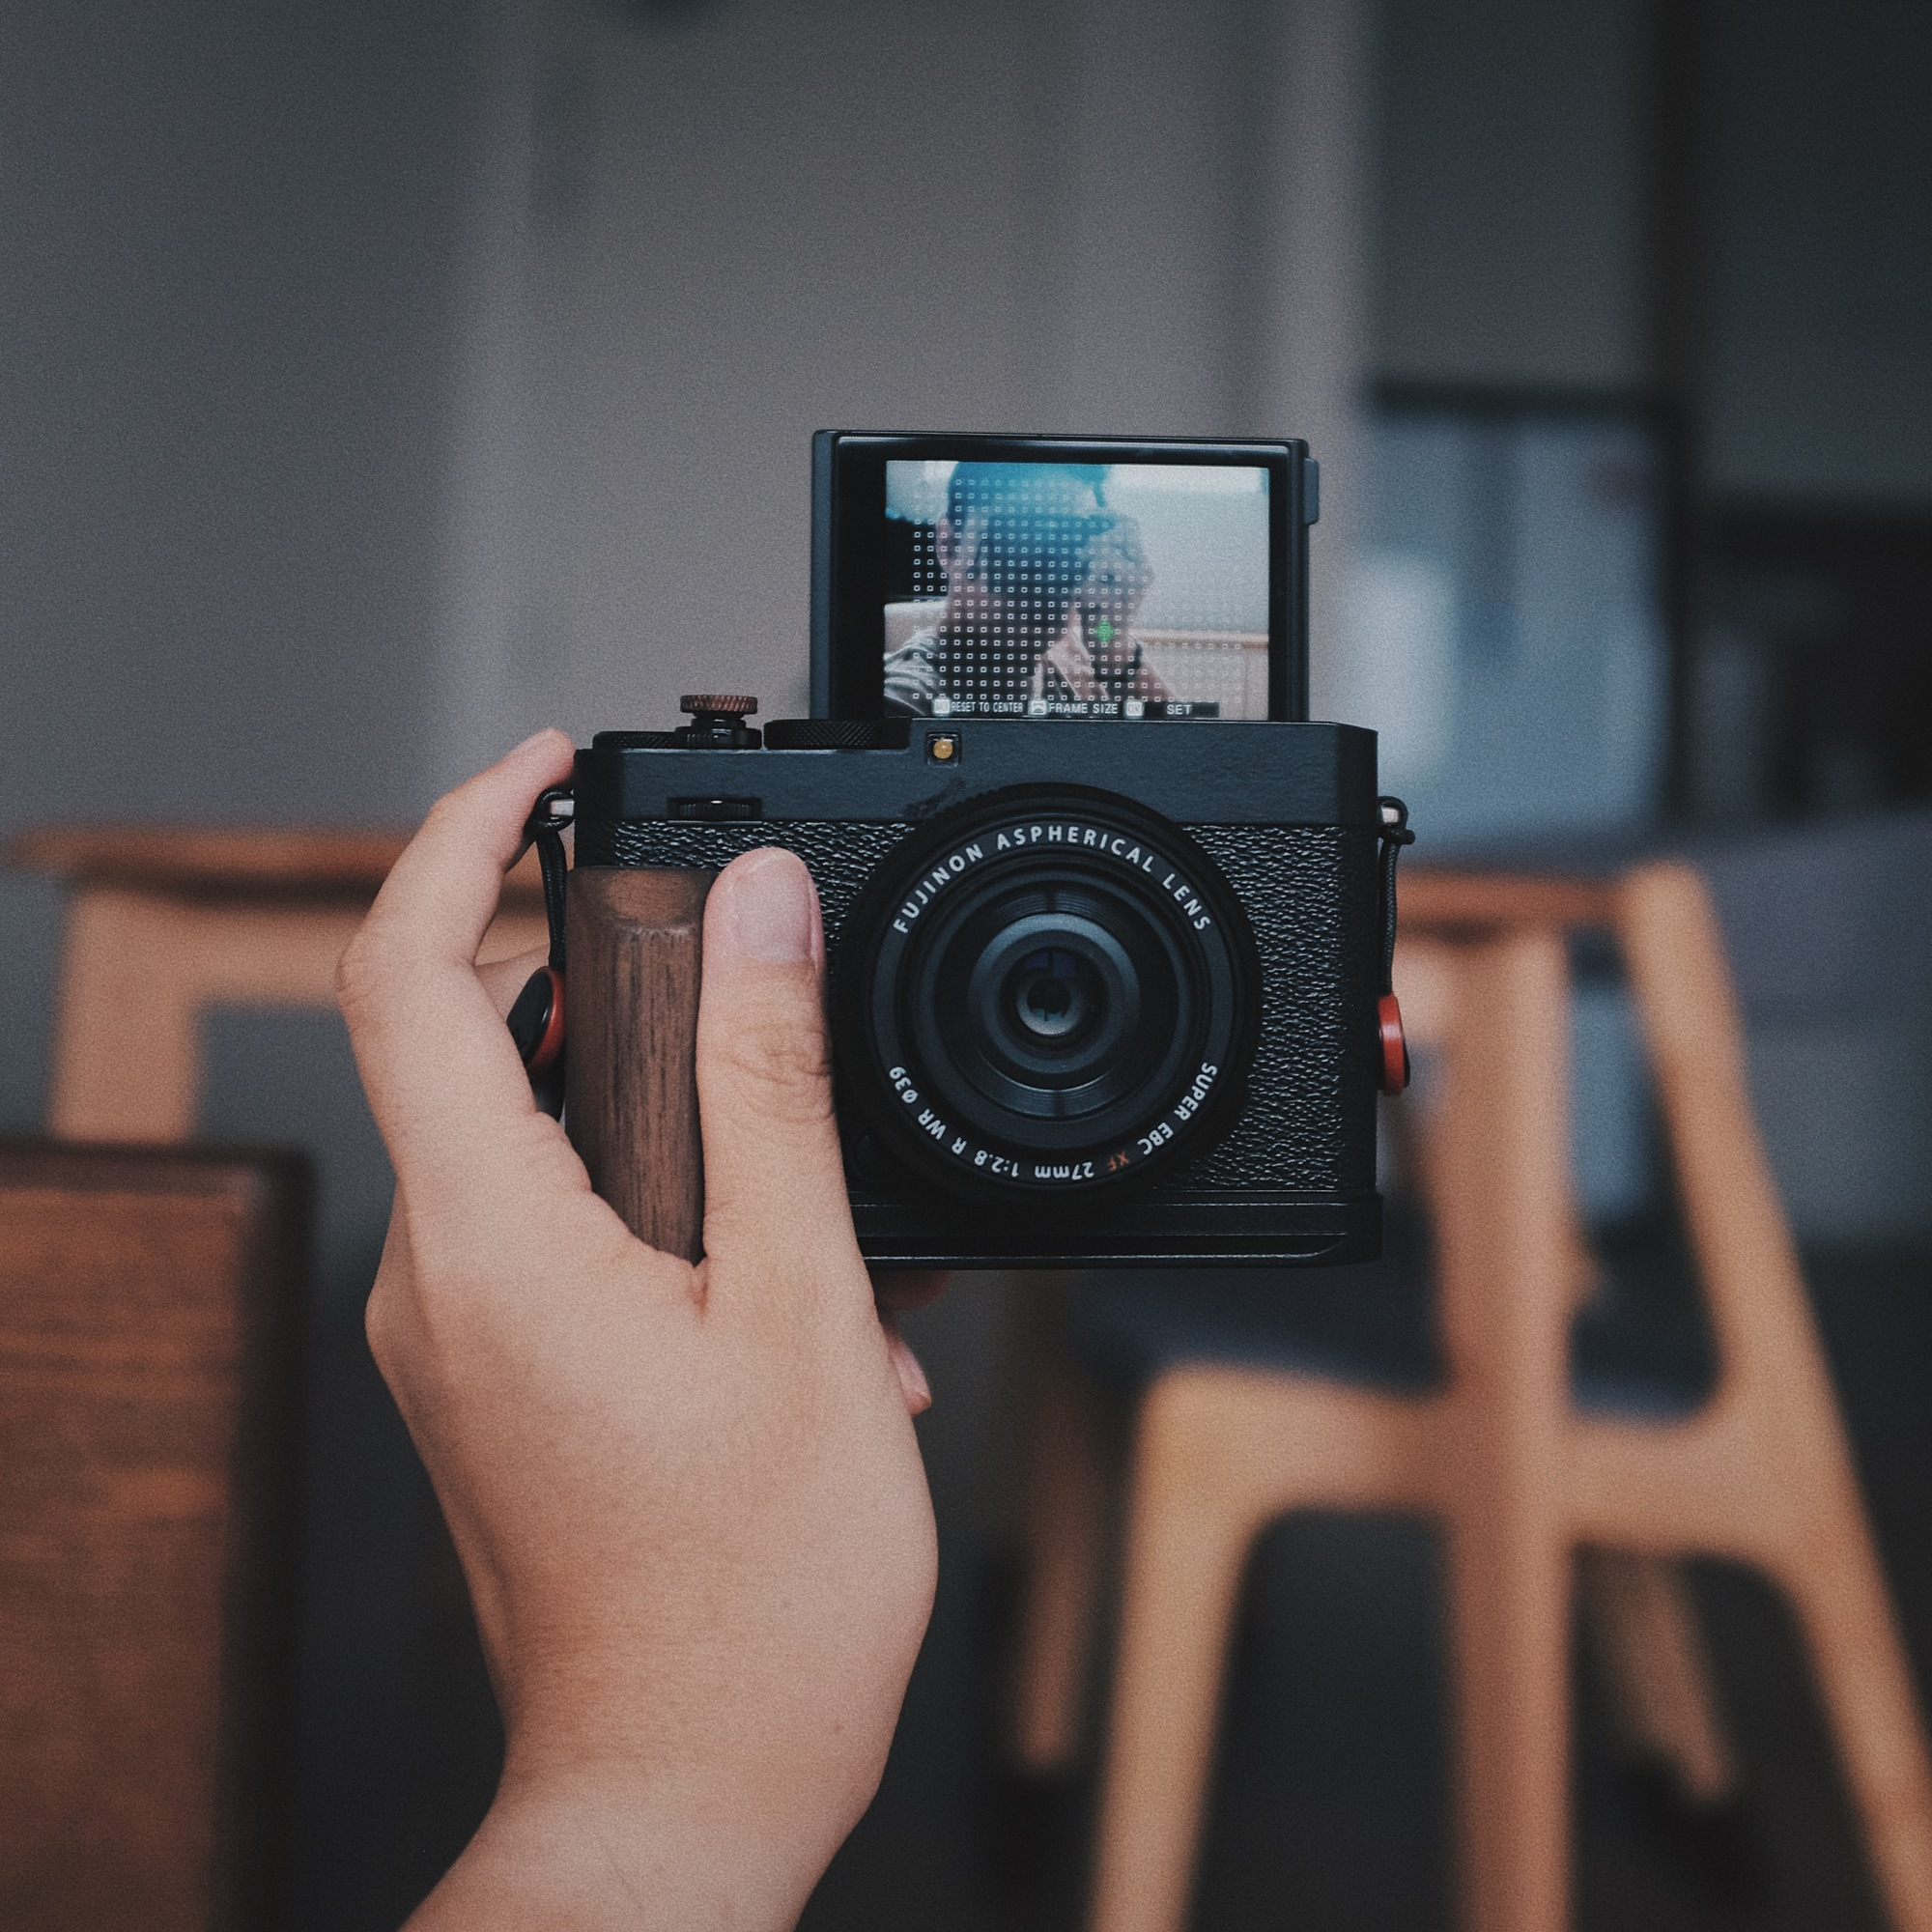
\includegraphics[width=\linewidth]{\envfinaldir/coverpic-prod.jpg}\par
            % \vskip 30pt
            \vfill

            \normalsize\rmfamily\scshape
            \copyright{} The Web Digest Project \hfill\large \envdatestr
        \end{center}
    \end{titlepage}
    % \restoregeometry
}
\newcommand{\simplehref}[1]{%
    \textcolor{blue!80!green}{\href{#1}{#1}}%
}
\renewcommand{\contentsname}{\center\Huge\sffamily\bfseries Contents\par\vskip 20pt}
\newcounter{ipartcounter}
\setcounter{ipartcounter}{0}
\newcommand{\ipart}[1]{
    % \vskip 20pt
    \clearpage
    \stepcounter{ipartcounter}
    \phantomsection
    \addcontentsline{toc}{chapter}{#1}
    % \begin{center}
    %     \Huge
    %     \sffamily\bfseries
    %     #1
    % \end{center}
    % \vskip 20pt plus 7pt
}
\newcounter{ichaptercounter}
\setcounter{ichaptercounter}{0}
\newcommand{\ichapter}[1]{
    % \vskip 20pt
    \clearpage
    \stepcounter{ichaptercounter}
    \phantomsection
    \addcontentsline{toc}{section}{\numberline{\arabic{ichaptercounter}}#1}
    \begin{center}
        \Huge
        \sffamily\bfseries
        #1
    \end{center}
    \vskip 20pt plus 7pt
}
\newcommand{\entrytitlefont}[1]{\subsection*{\raggedright\Large\sffamily\bfseries#1}}
\newcommand{\entryitemGeneric}[2]{
    % argv: title, url
    \parbox{\linewidth}{
        \entrytitlefont{#1}\par\vskip 5pt
        \footnotesize\ttfamily\mdseries
        \simplehref{#2}
    }\vskip 11pt plus 11pt minus 1pt
}
\newcommand{\entryitemGithub}[3]{
    % argv: title, url, desc
    \parbox{\linewidth}{
        \entrytitlefont{#1}\par\vskip 5pt
        \footnotesize\ttfamily\mdseries
        \simplehref{#2}\par\vskip 5pt
        \small\rmfamily\mdseries#3
    }\vskip 11pt plus 11pt minus 1pt
}
\newcommand{\entryitemAp}[3]{
    % argv: title, url, desc
    \parbox{\linewidth}{
        \entrytitlefont{#1}\par\vskip 5pt
        \footnotesize\ttfamily\mdseries
        \simplehref{#2}\par\vskip 5pt
        \small\rmfamily\mdseries#3
    }\vskip 11pt plus 11pt minus 1pt
}
\newcommand{\entryitemHackernews}[3]{
    % argv: title, hnurl, rawurl
    % \parbox{\linewidth}{
    %     \entrytitlefont{#1}\par\vskip 5pt
    %     \footnotesize\ttfamily\mdseries
    %     \simplehref{#3}\par
    %     \textcolor{black!50}{\href{#2}{#2}}
    % }\vskip 11pt plus 11pt minus 1pt
    \begin{minipage}{\linewidth}
            \entrytitlefont{#1}\par\vskip 5pt
            \footnotesize\ttfamily\mdseries
            \simplehref{#3}\par
            \textcolor{black!50}{\href{#2}{#2}}
    \end{minipage}\par\vskip 11pt plus 11pt minus 1pt
}







\begin{document}

\makeheader

\tableofcontents\clearpage




\ipart{Developers}
\ichapter{Hacker News}
\entryitemTwoLinks{Tesla sales drop for fifth month in a row in Europe}{https://news.ycombinator.com/item?id=44416780}{https://abcnews.go.com/Business/wireStory/europeans-angry-musk-buying-cars-tesla-sales-drop-123203026}

\entryitemTwoLinks{Many ransomware strains will abort if they detect a Russian keyboard installed (2021)}{https://news.ycombinator.com/item?id=44415233}{https://krebsonsecurity.com/2021/05/try-this-one-weird-trick-russian-hackers-hate/}

\entryitemTwoLinks{Tools I love: mise(-en-place)}{https://news.ycombinator.com/item?id=44414987}{https://blog.vbang.dk/2025/06/29/tools-i-love-mise/}

\entryitemTwoLinks{Loss of key US satellite data could send hurricane forecasting back 'decades'}{https://news.ycombinator.com/item?id=44414853}{https://www.theguardian.com/us-news/2025/jun/28/noaa-cuts-hurricane-forecasting-climate}

\entryitemTwoLinks{Personal care products disrupt the human oxidation field}{https://news.ycombinator.com/item?id=44414719}{https://www.science.org/doi/10.1126/sciadv.ads7908}

\entryitemTwoLinks{I made my VM think it has a CPU fan}{https://news.ycombinator.com/item?id=44413185}{https://wbenny.github.io/2025/06/29/i-made-my-vm-think-it-has-a-cpu-fan.html}

\entryitemTwoLinks{Bloom Filters by Example}{https://news.ycombinator.com/item?id=44412370}{https://llimllib.github.io/bloomfilter-tutorial/}

\entryitemTwoLinks{Show HN: Octelium – FOSS Alternative to Teleport, Cloudflare, Tailscale, Ngrok}{https://news.ycombinator.com/item?id=44412207}{https://github.com/octelium/octelium}

\entryitemTwoLinks{Using the Internet without IPv4 connectivity}{https://news.ycombinator.com/item?id=44411273}{https://jamesmcm.github.io/blog/no-ipv4/}

\entryitemTwoLinks{More on Apple's Trust-Eroding 'F1 the Movie' Wallet Ad}{https://news.ycombinator.com/item?id=44411069}{https://daringfireball.net/2025/06/more\_on\_apples\_trust-eroding\_f1\_the\_movie\_wallet\_ad}

\entryitemTwoLinks{The Unsustainability of Moore's Law}{https://news.ycombinator.com/item?id=44410900}{https://bzolang.blog/p/the-unsustainability-of-moores-law}

\entryitemTwoLinks{Blackwell: Nvidia's GPU}{https://news.ycombinator.com/item?id=44409391}{https://chipsandcheese.com/p/blackwell-nvidias-massive-gpu}

\entryitemTwoLinks{US Defense Department will stop providing satellite weather data}{https://news.ycombinator.com/item?id=44409175}{https://text.npr.org/nx-s1-5446120}

\entryitemTwoLinks{Solving `Passport Application` with Haskell}{https://news.ycombinator.com/item?id=44408872}{https://jameshaydon.github.io/passport/}

\entryitemTwoLinks{The Death of the Middle-Class Musician}{https://news.ycombinator.com/item?id=44408552}{https://thewalrus.ca/the-death-of-the-middle-class-musician/}

\entryitemTwoLinks{Schizophrenia is the price we pay for minds poised near the edge of a cliff}{https://news.ycombinator.com/item?id=44408286}{https://www.psychiatrymargins.com/p/schizophrenia-is-the-price-we-pay}

\entryitemTwoLinks{2025 ARRL Field Day}{https://news.ycombinator.com/item?id=44407245}{https://www.arrl.org/field-day}

\entryitemTwoLinks{JavaScript Trademark Update}{https://news.ycombinator.com/item?id=44407139}{https://deno.com/blog/deno-v-oracle4}

\entryitemTwoLinks{Life of an inference request (vLLM V1): How LLMs are served efficiently at scale}{https://news.ycombinator.com/item?id=44407058}{https://www.ubicloud.com/blog/life-of-an-inference-request-vllm-v1}

\entryitemTwoLinks{Use Plaintext Email (2019)}{https://news.ycombinator.com/item?id=44406837}{https://useplaintext.email/}


\ipart{Developers~~~~(zh-Hans)}
\ichapter{Solidot}
\entryitemGeneric{\hskip 0pt{}Canonical 2024 年营收 2.92 亿美元}{https://www.solidot.org/story?sid=81676}

\entryitemGeneric{\hskip 0pt{}研究发现白垩纪海洋是``乌贼的天下''}{https://www.solidot.org/story?sid=81675}

\entryitemGeneric{\hskip 0pt{}日本争议夫妇别姓法案}{https://www.solidot.org/story?sid=81674}

\entryitemGeneric{\hskip 0pt{}中国平面设计师面临 AI 图像生成器的挑战}{https://www.solidot.org/story?sid=81673}

\entryitemGeneric{\hskip 0pt{}Bcachefs 文件系统可能将会移除出内核}{https://www.solidot.org/story?sid=81672}

\entryitemGeneric{\hskip 0pt{}德国要求苹果和 Google 下架 DeepSeek}{https://www.solidot.org/story?sid=81671}

\entryitemGeneric{\hskip 0pt{}微软用黑屏死机替代蓝屏死机}{https://www.solidot.org/story?sid=81670}

\entryitemGeneric{\hskip 0pt{}笑声也会感染倭黑猩猩}{https://www.solidot.org/story?sid=81669}

\entryitemGeneric{\hskip 0pt{}数字主权始于桌面:欧洲 Linux 桌面时代有望到来}{https://www.solidot.org/story?sid=81668}

\entryitemGeneric{\hskip 0pt{}AMD 成为 Debian 开发者大会的白金赞助商}{https://www.solidot.org/story?sid=81667}

\entryitemGeneric{\hskip 0pt{}丹麦以赋权公民的方式打击深度伪造}{https://www.solidot.org/story?sid=81666}

\entryitemGeneric{\hskip 0pt{}当美国人遇到新闻付费墙很少有人愿意付费}{https://www.solidot.org/story?sid=81665}

\entryitemGeneric{\hskip 0pt{}研究发现大模型用户理解能力较弱}{https://www.solidot.org/story?sid=81664}

\entryitemGeneric{\hskip 0pt{}微软正将杀毒软件移出 Windows 内核}{https://www.solidot.org/story?sid=81663}

\entryitemGeneric{\hskip 0pt{}Google DeepMind 发布 AlphaGenome}{https://www.solidot.org/story?sid=81662}

\entryitemGeneric{\hskip 0pt{}美国计算机科学专业入学人数出现下降趋势}{https://www.solidot.org/story?sid=81661}\ichapter{V2EX}
\entryitemGeneric{\hskip 0pt{}[分享发现] 幽门螺杆菌引起的肠胃型口臭}{https://www.v2ex.com/t/1141843}

\entryitemGeneric{\hskip 0pt{}[智能家电] 普通挂机空调有第三方线控器接入米家吗?}{https://www.v2ex.com/t/1141842}

\entryitemGeneric{\hskip 0pt{}[分享创造] (公益)在线订阅转换工具 - 自建一个属于你的订阅转换系统,告别订阅链接泄露,前端与后端部署教程}{https://www.v2ex.com/t/1141840}

\entryitemGeneric{\hskip 0pt{}[问与答] 国内大模型与 chatgpt}{https://www.v2ex.com/t/1141839}

\entryitemGeneric{\hskip 0pt{}[问与答] 好的 c++代码是什么样的}{https://www.v2ex.com/t/1141838}

\entryitemGeneric{\hskip 0pt{}[分享发现] 豆包否定岳飞是民族英雄, deepseek 却认为岳飞是民族英雄}{https://www.v2ex.com/t/1141837}

\entryitemGeneric{\hskip 0pt{}[健康] 匿名体检/基因组测序}{https://www.v2ex.com/t/1141835}

\entryitemGeneric{\hskip 0pt{}[问与答] ios 端任何浏览器打开 github 样式都是错乱的}{https://www.v2ex.com/t/1141833}

\entryitemGeneric{\hskip 0pt{}[问与答] 看 nas 的视频的时候想看弹幕怎么办,用的是飞牛 OS}{https://www.v2ex.com/t/1141832}

\entryitemGeneric{\hskip 0pt{}[VPS] CloudCone 是不是又挂了.....}{https://www.v2ex.com/t/1141831}

\entryitemGeneric{\hskip 0pt{}[全球工单系统] CloudCone 疑似大面积宕机}{https://www.v2ex.com/t/1141830}

\entryitemGeneric{\hskip 0pt{}[分享创造] 开源了一个现代化照片画廊网站 - Afilmory}{https://www.v2ex.com/t/1141829}

\entryitemGeneric{\hskip 0pt{}[VPS] 带原邮出搬瓦工 CN2 GIA The DC9 Plan VPS 一只}{https://www.v2ex.com/t/1141828}

\entryitemGeneric{\hskip 0pt{}[Cursor] Cursor 200 美金的 Ultra 好像没有 25 次工具调用次数限制了}{https://www.v2ex.com/t/1141827}

\entryitemGeneric{\hskip 0pt{}[分享创造] 自己写了个工具:测试各种 LLM 接口性能,专治那些``说得好听但跑得慢''的 AI 中转站}{https://www.v2ex.com/t/1141826}

\entryitemGeneric{\hskip 0pt{}[分享发现] 噗!``类型弱置''}{https://www.v2ex.com/t/1141825}

\entryitemGeneric{\hskip 0pt{}[随想] 文字, 规则, 一切形式是人的序列化}{https://www.v2ex.com/t/1141824}

\entryitemGeneric{\hskip 0pt{}[问与答] 微信多条消息的点击问题}{https://www.v2ex.com/t/1141822}

\entryitemGeneric{\hskip 0pt{}[Swift] FoundationModels 框架实践}{https://www.v2ex.com/t/1141821}

\entryitemGeneric{\hskip 0pt{}[硬件] 自动控制原理}{https://www.v2ex.com/t/1141819}

\entryitemGeneric{\hskip 0pt{}[推广] 兄弟姐妹们薅羊毛了,新的企业信息查询网站,注册薅 5 年 SVIP。}{https://www.v2ex.com/t/1141818}

\entryitemGeneric{\hskip 0pt{}[分享创造] 写了一个导出管理 AI 对话记录的 React 应用}{https://www.v2ex.com/t/1141817}

\entryitemGeneric{\hskip 0pt{}[随想] 再也不会碰到那样的女孩}{https://www.v2ex.com/t/1141816}

\entryitemGeneric{\hskip 0pt{}[音乐] 那些年他们翻唱过的中岛美雪 - Apple Music 中国大陆区歌单}{https://www.v2ex.com/t/1141815}

\entryitemGeneric{\hskip 0pt{}[问与答] 求助,一个局域网内的 im!}{https://www.v2ex.com/t/1141814}

\entryitemGeneric{\hskip 0pt{}[Apple] 为了消耗电池健康度,用 AI 开发了 app——``Roar''}{https://www.v2ex.com/t/1141813}

\entryitemGeneric{\hskip 0pt{}[Apple] MacOS 26 目前做开发还有什么坑吗?}{https://www.v2ex.com/t/1141812}

\entryitemGeneric{\hskip 0pt{}[问与答] 连锁式机场置换充电宝服务如何?}{https://www.v2ex.com/t/1141811}

\entryitemGeneric{\hskip 0pt{}[问与答] 有人搞抖音自媒体副业吗?有没有人教我一下怎么避免审核问题?}{https://www.v2ex.com/t/1141809}

\entryitemGeneric{\hskip 0pt{}[程序员] 尝试做了一个 tauri 的客户端项目,并且分享一下最近参加 cursor 中国社区举办的活动经历}{https://www.v2ex.com/t/1141808}

\entryitemGeneric{\hskip 0pt{}[问与答] 个人开发者如何推广自己开发的小程序}{https://www.v2ex.com/t/1141807}

\entryitemGeneric{\hskip 0pt{}[分享发现] [教程]一个服务器安装了 frps,占用了 80、443 端口,怎么继续使用 80、443 端口建站呢? 一个解决办法}{https://www.v2ex.com/t/1141806}

\entryitemGeneric{\hskip 0pt{}[奇思妙想] 游戏相关点子,欢迎来喷}{https://www.v2ex.com/t/1141805}

\entryitemGeneric{\hskip 0pt{}[问与答] Windows11,触控板手势客制化程序推荐}{https://www.v2ex.com/t/1141804}

\entryitemGeneric{\hskip 0pt{}[宽带症候群] 安徽电信晚高峰 Q 麻了}{https://www.v2ex.com/t/1141803}

\entryitemGeneric{\hskip 0pt{}[推广] 纪念一下第一次收到开源赞助}{https://www.v2ex.com/t/1141801}

\entryitemGeneric{\hskip 0pt{}[健康] 等牙疼好了,再去拔智齿.}{https://www.v2ex.com/t/1141800}

\entryitemGeneric{\hskip 0pt{}[分享创造] 🚀开源 AI 联网搜索工具: Open-WebSearch MCP 全新升级,支持多引擎 + 流式响应!}{https://www.v2ex.com/t/1141799}

\entryitemGeneric{\hskip 0pt{}[创业组队] 寻找靠谱创业团队/靠谱合伙人}{https://www.v2ex.com/t/1141798}

\entryitemGeneric{\hskip 0pt{}[问与答] 请各位 V 友出出主意,如何对付无良中介和房东?}{https://www.v2ex.com/t/1141797}

\entryitemGeneric{\hskip 0pt{}[分享发现] Edge 新版本更新了 AI 转译音频功能}{https://www.v2ex.com/t/1141796}

\entryitemGeneric{\hskip 0pt{}[宽带症候群] 家宽有 80 和 443,宝塔搭建什么好玩?}{https://www.v2ex.com/t/1141795}

\entryitemGeneric{\hskip 0pt{}[健康] 我的鼾症严重到要上呼吸机了,想咨询一下大家}{https://www.v2ex.com/t/1141793}

\entryitemGeneric{\hskip 0pt{}[Google] gv 号收不到纸飞机验证码}{https://www.v2ex.com/t/1141792}

\entryitemGeneric{\hskip 0pt{}[问与答] 想买个可解锁的安卓机,暂定 OP13T,哪个渠道比较便宜呢}{https://www.v2ex.com/t/1141791}

\entryitemGeneric{\hskip 0pt{}[程序员] claude code 的服从性远不如 cursor}{https://www.v2ex.com/t/1141790}

\entryitemGeneric{\hskip 0pt{}[MacBook Pro] Macbook Pro 屏幕出现淡淡的回字形条纹}{https://www.v2ex.com/t/1141789}

\entryitemGeneric{\hskip 0pt{}[iPhone] 蛋疼,感觉现在买带 mfi 的 L 口充电线是在浪费钱}{https://www.v2ex.com/t/1141787}

\entryitemGeneric{\hskip 0pt{}[程序员] 程序员的第一个 NAS: 采用 N150 的 1100 元的 6 盘位 NAS}{https://www.v2ex.com/t/1141786}

\entryitemGeneric{\hskip 0pt{}[分享创造] 花了两小时做了一个 cd calculator 在线计算器}{https://www.v2ex.com/t/1141785}


\ipart{Generic News}







\clearpage
\leavevmode\vfill
\footnotesize

Copyright \copyright{} 2023-2025 Neruthes and other contributors.

This document is published with CC BY-NC-ND 4.0 license.

The entries listed in this newsletter may be copyrighted by their respective creators.

This newsletter is generated by the Web Digest project.

The newsletters are also delivered via Telegram channel \CJKunderline{\href{https://t.me/webdigestchannel}{https://t.me/webdigestchannel}}.\\
RSS feed is available at \CJKunderline{\href{https://webdigest.pages.dev/rss.xml}{https://webdigest.pages.dev/rss.xml}}.

This newsletter is available in PDF at
\CJKunderline{\href{https://webdigest.pages.dev/}{https://webdigest.pages.dev/}}.

The source code being used to generate this newsletter is available at\\
\CJKunderline{\href{https://github.com/neruthes/webdigest}{https://github.com/neruthes/webdigest}}.

This newsletter is also available in
\CJKunderline{\href{http://webdigest.pages.dev/readhtml/\envyear/WebDigest-20250630.html}{HTML}} and
\CJKunderline{\href{https://github.com/neruthes/webdigest/blob/master/markdown/\envyear/WebDigest-20250630.md}{Markdown}}.


\coverpic{https://unsplash.com/photos/rQQ8tWZnHFY}{BHLNZ - Biodiversity Heritage Library NZ}


\end{document}
